\documentclass[notes,serif]{beamer}
\usepackage{graphicx}
\usepackage{url}
\usepackage{clrscode}
\usepackage{amssymb,amsmath}

% You should run 'pdflatex' TWICE, because of TOC issues.

\mode<presentation>
{
  % A tip: pick a theme you like first, and THEN modify the color theme, and then add math content.
  % Warsaw is the theme selected by default in Beamer's installation sample files.

  %%%%%%%%%%%%%%%%%%%%%%%%%%%% THEME
  %\usetheme{AnnArbor}
  %\usetheme{Antibes}
  %\usetheme{Bergen}
  %\usetheme{Berkeley}
  %\usetheme{Berlin}
  %\usetheme{Boadilla}
  %\usetheme{boxes}
  %\usetheme{CambridgeUS}
  %\usetheme{Copenhagen}
  %\usetheme{Darmstadt}
  %\usetheme{default}
  %\usetheme{Dresden}
  %\usetheme{Frankfurt}
  %\usetheme{Goettingen}
  %\usetheme{Hannover}
  %\usetheme{Ilmenau}
  %\usetheme{JuanLesPins}
  %\usetheme{Luebeck}
  %\usetheme{Madrid}
  %\usetheme{Malmoe}
  %\usetheme{Marburg}
  %\usetheme{Montpellier}
  %\usetheme{PaloAlto}
  %\usetheme{Pittsburgh}
  %\usetheme{Rochester}
  %\usetheme{Singapore}
  %\usetheme{Szeged}
  \usetheme{Warsaw}

  %%%%%%%%%%%%%%%%%%%%%%%%%%%% COLOR THEME
  %\usecolortheme{albatross}
  %\usecolortheme{beetle}
  %\usecolortheme{crane}
  \usecolortheme{default}
  %\usecolortheme{dolphin}
  %\usecolortheme{dove}
  %\usecolortheme{fly}
  %\usecolortheme{lily}
  %\usecolortheme{orchid}
  %\usecolortheme{rose}
  %\usecolortheme{seagull}
  %\usecolortheme{seahorse}
  %\usecolortheme{sidebartab}
  %\usecolortheme{structure}
  %\usecolortheme{whale}

  %%%%%%%%%%%%%%%%%%%%%%%%%%%% OUTER THEME
  %\useoutertheme{default}
  %\useoutertheme{infolines}
  %\useoutertheme{miniframes}
  %\useoutertheme{shadow}
  %\useoutertheme{sidebar}
  %\useoutertheme{smoothbars}
  %\useoutertheme{smoothtree}
  %\useoutertheme{split}
  %\useoutertheme{tree}

  %%%%%%%%%%%%%%%%%%%%%%%%%%%% INNER THEME
  %\useinnertheme{circles}
  %\useinnertheme{default}
  %\useinnertheme{inmargin}
  %\useinnertheme{rectangles}
  %\useinnertheme{rounded}

  %%%%%%%%%%%%%%%%%%%%%%%%%%%%%%%%%%%

%  \setbeamercovered{transparent} % or whatever (possibly just delete it)
  \setbeamercovered{invisible} % or whatever (possibly just delete it)
  % To change behavior of \uncover from graying out to totally invisible, can change \setbeamercovered to invisible instead of transparent. apparently there are also 'dynamic' modes that make the amount of graying depend on how long it'll take until the thing is uncovered.

}


% Get rid of nav bar
\beamertemplatenavigationsymbolsempty

% Use short top
%\usepackage[headheight=12pt,footheight=12pt]{beamerthemeboxes}
%\addheadboxtemplate{\color{black}}{
%\hskip0.3cm
%\color{white}
%\insertshortauthor \ \ \ \
%\insertframenumber \ \ \ \ \ \ \
%\insertsection \ \ \ \ \ \ \ \ \ \ \ \ \ \ \ \ \  \insertsubsection
%\hskip0.3cm}
%\addheadboxtemplate{\color{black}}{
%\color{white}
%\ \ \ \
%\insertsection
%}
%\addheadboxtemplate{\color{black}}{
%\color{white}
%\ \ \ \
%\insertsubsection
%}

% Insert frame number at bottom of the page.
\usefoottemplate{\hfil\tiny{\color{black!90}\insertframenumber}}

\usepackage[english]{babel}
\usepackage[latin1]{inputenc}

\usepackage{times}
\usepackage[T1]{fontenc}

\title{Design and Analysis of Algorithms}
\subtitle{Lecture 3---Randomized Algorithms}

\author{Lei Wang}

\institute{Dalian University of Technology}

%\date{Date}

\subject{Talks}

\def\defn#1{{\color{red} #1}}

\begin{document}

\begin{frame}
  \titlepage
\end{frame}

\begin{frame}
  \frametitle{Probabilistic Analysis and Randomized Algorithms}
  \tableofcontents
\end{frame}

\section{Overview}
\subsection{Goals}

\begin{frame}
\frametitle{Goals}
\begin{itemize}
    \item Explain the difference between probabilistic analysis and randomized algorithms,
    \item present the technique of indicator random variables, and
    \item give another example of the analysis of a randomized algorithm (permuting an array in place).
\end{itemize}

%Preliminary things that we must cover before going on:
%
%\begin{columns}
%
%\column{0.5\textwidth}
%
%Working inside a column...
%
%\begin{block}{Blocks default to blue}
%\begin{itemize}
%\item Itemize
%\item Itemize
%\end{itemize}
%\end{block}
%
%\begin{alertblock}{Alert Blocks are red (by default)}
%\begin{enumerate}
%\item Enumerate
%\item Enumerate
%\end{enumerate}
%\end{alertblock}
%
%\column{0.5\textwidth}
%
%\hyperlink{post_equalities}{\beamergotobutton{Skip rest of $\mathbb{R}^{n+1}$}}
%
%This is a precursor to studying \defn{integrals}:
%\begin{equation*}
%\int_a^b f(x)\ dx
%\end{equation*}
%
%\begin{exampleblock}{Example blocks for green}
%\begin{equation}
%\sum_{i=1}^\infty \frac1{n^2} = \frac\pi6
%\end{equation}
%\end{exampleblock}
%
%\pause\uncover{
%  This is a pause/uncover...\footnote{Use them for ``animation'' effect.}
%}
%
%%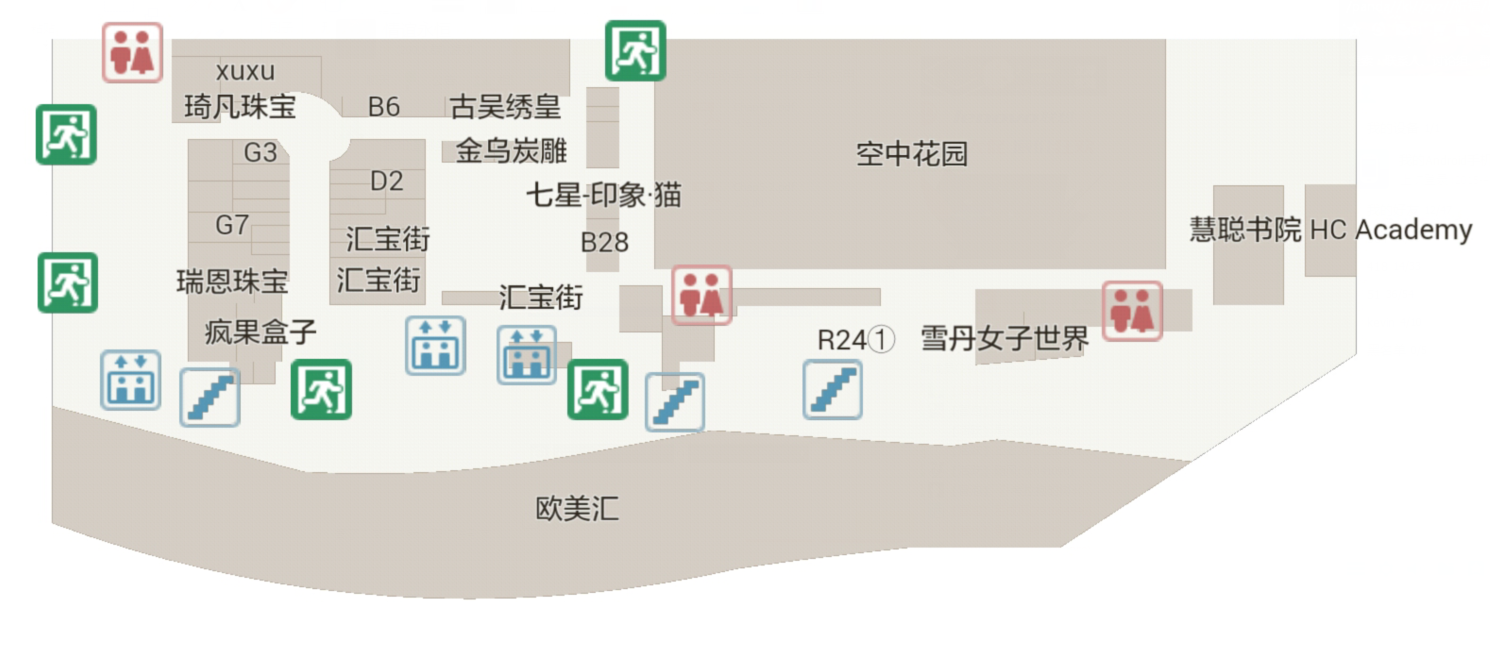
\includegraphics[width=2in]{example.jpg}
%
%\end{columns}
%
\end{frame}

%\subsection{Subsection 2}
%
%\begin{frame}
%\frametitle{Themes and TOC Space-Budgeting Issues}
%
%\hypertarget{post_equalities}{}
%
%A comment: I put all of these generically-named sections and subsections so that you can see what the different themes do to them.  If you happen to have a lot of sections and subsections (for example), then the Warsaw theme tends to take up a lot of space at the top.
%\begin{itemize}
%\item You can uncomment some code I have near the top that will just show the CURRENT section/subsection
%\item Or, if you don't like that, try using a theme that has the TOC run down a left-hand or right-hand column.  What you lose horizontally, you gain vertically.
%\end{itemize}
%
%\end{frame}
%
%\subsection{Subsection 3}
%
%\begin{frame}
%\frametitle{On Frame Titles}
%
%Good form apparently dictates that frames are supposed to have a title.  Titles should be informative.  ``Proof of Riemann Hypothesis'' beats ``Proof'' as a frame title (just in case an audience member zoned out at some point).
%
%\end{frame}

\section{The Hiring Problem}

\subsection{The hiring problem}

\begin{frame}
  \frametitle{The hiring problem}
  \begin{block}{\bf Scenario:}
    \begin{itemize}
      \item You are using an employment agency to hire a new office assistant.
      \item The agency sends you one candidate each day.
      \item You interview the candidate and must immediately decide whether or not to
hire that person.  But if you hire, you must also fire your current office assistant even if it's someone you have recently hired.
      \item Cost to interview is $c_i$ per candidate (interview fee paid to agency).
      \item Cost to hire is $c_h$ per candidate (includes cost to fire current office assistant + hiring fee paid to agency).
      \item You are committed to having hired, at all times, the best candidate seen so far.
    \end{itemize}
  \end{block}
\end{frame}

\begin{frame}
  \frametitle{The hiring problem (cont.)}
  \begin{alertblock}{\bf Goal}
    {\bf Determine what the price of this strategy will be.} \\
    {\bf \em Pseudocode to model this scenario:}  Assumes that the candidates are numbered $1$ to $n$ and that after interviewing each candidate, we can determine if it's better than the current office assistant.
  \end{alertblock}
  \begin{block}{\textsc{Hire-Assistant($n$)}}
    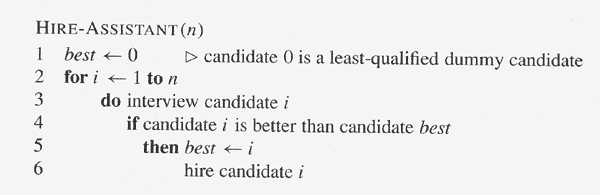
\includegraphics[height=3.5cm]{05-hire_assistant}
  \end{block}
\end{frame}

\subsection{The cost}
\begin{frame}
  \frametitle{The cost}
  If $n$ candidates, and we hire $m$ of them, the cost is $O(nc_i + mc_h)$.
  \begin{itemize}
    \item Have to pay $nc_i$ to interview, no matter how many we hire.
    \item So we focus on analyzing the hiring cost $mc_h$.
    \item $mc_h$ varies with each run---it depends on the order in which we interview the candidates.
    \item This is a model of a common paradigm: we need to find the maximum or minimum in a sequence by examining each element and maintaining a current ``winner.'' The variable m denotes how many times we change our notion of which element is currently winning.
  \end{itemize}
\end{frame}

\subsection{Worst-case Analysis}
\begin{frame}
\frametitle{Worst-case analysis}
  \begin{itemize}
    \item In the worst case, we hire all $n$ candidates.
    \item This happens if each one is better than all who came before.  In other words, \pause \uncover {if the candidates appear in increasing order of quality.}
    \pause
    \item If we hire all $n$, then the cost is $O(nc_i + nc_h) = O(nc_h)$ (since $c_h > c_i$ ).
  \end{itemize}
\end{frame}

\subsection{Probabilistic analysis}
\begin{frame}
  \frametitle{Probabilistic analysis}
  In general, we have no control over the order in which candidates appear.
  We could assume that they come in a random order:
  \begin{itemize}
    \item Assign a rank to each candidate: $rank(i)$ is a unique integer in the range $1$ to $n$.
    \item The ordered list $\langle rank(1), rank(2), \dots , rank(n)\rangle$ is a permutation of the candidate numbers $\langle 1, 2, \dots , n \rangle$.
    \item The list of ranks is equally likely to be any one of the $n!$ permutations.
    \item Equivalently, the ranks form a {\bf \em uniform random permutation}: each of the possible
$n!$ permutations appears with equal probability.
  \end{itemize}
\end{frame}

\section{Randomized Algorithms}
\subsection{Randomized algorithms}
\begin{frame}
\frametitle{Randomized algorithms}
    We might not know the distribution of inputs, or we might not be able to model it computationally.  Instead, we use randomization within the algorithm in order to impose a distribution on the inputs.
  \begin{block}{{\bf \em For the hiring problem:} Change the scenario:}
  \begin{itemize}
    \item The employment agency sends us a list of all $n$ candidates in advance.
    \item On each day, we randomly choose a candidate from the list to interview (but considering only those we have not yet interviewed).
    \item Instead of relying on the candidates being presented to us in a random order, we take control of the process and enforce a random order.
  \end{itemize}
  \end{block}
\end{frame}

\begin{frame}
\frametitle{Randomized algorithms (cont.)}
  \begin{block}{{\bf \em What makes an algorithm randomized:}}
  An algorithm is randomized if its behavior is determined in part by values produced by a random-number generator.
  \begin{itemize}
    \item \textsc{Random}$(a, b)$ returns an integer $r$, where $a \le r \le b$ and each of the $b-a+1$ possible values of $r$ is equally likely.
    \item In practice, \textsc{{R}andom} is implemented by a {\bf \em pseudorandom-number generator}, which is a deterministic method returning numbers that {\color{blue}``look''} random and pass statistical tests.
  \end{itemize}
  \end{block}
\end{frame}

\subsection{Indicator Random Variables}
\begin{frame}
\frametitle{Indicator random variables}
Given a sample space and an event $A$, we define the {\bf \em indicator random variable}
$$
I\{A\}=
\begin{cases}
1 & \text{if $A$ occurs,} \\
0 & \text{if $A$ does not occur.}
\end{cases}
$$
  \begin{block}{\bf \em Lemma}
    For an event $A$, let $X_A = I\{A\}$. Then $E[X_A] = \text{Pr}\{A\}$. \\
    {\bf \em Proof} Letting $\overline{A}$ be the complement of $A$, we have
    \begin{align*}
      E[X_A] &= E[I\{A\}] \\
                   &= 1 \cdot \text{Pr} \{A\} + 0 \cdot \text{Pr} \{\overline{A}\}  & & \text{(definition of expected value)} \\
                   &= \text{Pr} \{A\}.
    \end{align*}
  \end{block}
Some examples...
\end{frame}

\subsection{Analysis of the hiring problem}
\begin{frame}
\frametitle{Analysis of the hiring problem}
Assume that the candidates arrive in a random order.  Let $X$ be a random variable that equals the number of times we hire a new office assistant.  Define indicator random variables $X_1, X_2, \dots , X_n$, where $X_i = I\{\text{candidate $i$ is hired}\}$.

\begin{block}{\bf \em Useful properties:}
  \begin{itemize}
    \item $X = X_1 + X_2 + \cdots + X_n$.
    \item {\bf Lemma} $\Rightarrow E[X_i] = \text{Pr}\{\text{candidate $i$ is hired}\}$.
    \item Pr\{candidate $i$ is the best so far\} $= 1/i$, which implies $E[X_i] = 1/i$.
    \item we can get \\
      $ E[X] = E [ \sum_{i=1}^n X_i ] = \sum_{i=1}^nE[X_i ] = \sum_{i=1}^n 1/i = \text{ln}n + O(1) $
      $ \Rightarrow \mbox { the expected hiring cost } O(c_h \cdot \text{ln}n), \mbox{\color{red} much better than } O(c_h n).
      $
  \end{itemize}
\end{block}
\end{frame}

\end{document} 